\chapter{INTRODUCTION} \label{chap:one}
	What is presented in this thesis is an abstraction. We seek to encapsulate a sufficient amount of information about fibers on a scale small enough to realistically incorporate short-range forces, specifically intermolecular forces are considered. A strong focus on carbon nanotubes is used because they were a motivation but also they are appropriate to fit the abstraction and thus give a good frame of reference. The introduction continues with:

\begin{itemize}	
	\item {
		brief history and anthology of graphene and carbon nanotubes, 
	}
	\item {
		a discussion of experimental materials involving several fibers,
	}
	\item {
		models for those materials,
	}
	\item {
		models for similar materials also involving adhesion,
	}
	\item {
		and a summary of the rest of the thesis.
	}
\end{itemize}



\section{Graphene and carbon nanotubes}
	
	Graphene is a hexagonal lattice of covalently bonded carbon atoms. Thought of as a two dimensional crystalline lattice, graphene is known to be a structural component to graphite, carbon nanotubes, and other materials. However, the existence of stable graphene sheets was only speculative until they were isolated experimentally in 2004 \cite{Novoselov2004}. Graphene has many potential applications primarily because of the high Young's modulus, room temperature electron mobility, thermal conductivity, optical absorption, gas impermeability, etc \cite{Novoselov2012}. Recently developed novel transistors \cite{Lin2010} and composite materials for solar cells \cite{Wang2013} emphasize the future promise of graphene. Mass production of an acceptable quality of graphene is, however, still in its infancy, and with it so are industrial applications \cite{Novoselov2012}.
	
	\begin{figure}
		\begin{center}
			\def\svgwidth{.75\columnwidth}
			\input{./old_fig/Chirality.eps_tex}
		\end{center}		
		\caption{A graphene sheet with possible choices of a chiral vector $\mbox{C}_{\textbf{v}}$.
		\label{fig:GrapheneCat}}
	\end{figure}	
	
	Carbon nanotubes were first identified in 1950's although they were brought to the attention of the wider scientific community in 1991 \cite{Iijima1991}. A carbon nanotube (CNT) can conceptually be thought of as an appropriately rolled graphene lattice (see Fig.~\ref{fig:GrapheneCat}). CNTs are categorized by their chirality and the number of encasing shells. A CNT is called a single-walled carbon nanotube (SWCNT) if there is only one cylindrical structure with no additional interior or exterior CNTs, a double-walled carbon nanotube (DWCNT) if there is exactly two concentric CNTs, or a multi-walled carbon nanotube (MWCNT) if there are more than two. Chirality of a CNT is categorized by a vector on a graphene sheet. The basis for this vector is shown on Fig.~\ref{fig:GrapheneCat}, $a_1$ and $a_2$, which forces head and tail points to lie on vertices of a hexagon. A CNT is then formed by rolling the graphene sheet along the vector, $\mbox{C}_{\textbf{v}}$, until the head and tail points meet. In this way $\mbox{C}_{\textbf{v}}$ determines the circumference of the CNT and an orthogonal vector T is the tube axis. The tail is usually taken as a reference or origin point, and then chirality is determined by the position of the head. A CNT is called armchair if along the tube axis the hexagon structure repeats uniformly (see Fig.~\ref{subfig:Armchair}), zigzag if the hexagon structure alternates (see Fig.~\ref{subfig:Zigzag}), and chiral otherwise.
	
	Like graphene, CNTs have many desirable properties. In particular, depending on the structure of a CNT, a tube behaves either as a semiconductor or a metal, has an effective Young's modulus comparable to graphene, and has unique thermal conductivity \cite{Dresselhaus2004}. Both graphene and CNTs have strong molecular bonds between carbon atoms which makes them strong under tension, but each bond allows small deformations which can lead to a large curvature. Moreover, under heavy strain CNTs can relax via Stone-Walls diatomic interchange creating sharper bends and deformation \cite{Yakobson1998}. CNTs are already being used in industrial applications from lithium ion batteries to composite bicycle frames \cite{De2013} with future applications being researched.
	
	\begin{figure*}[t!]
		\centering
		\begin{subfigure}[t]{.5\textwidth}
			\centering
			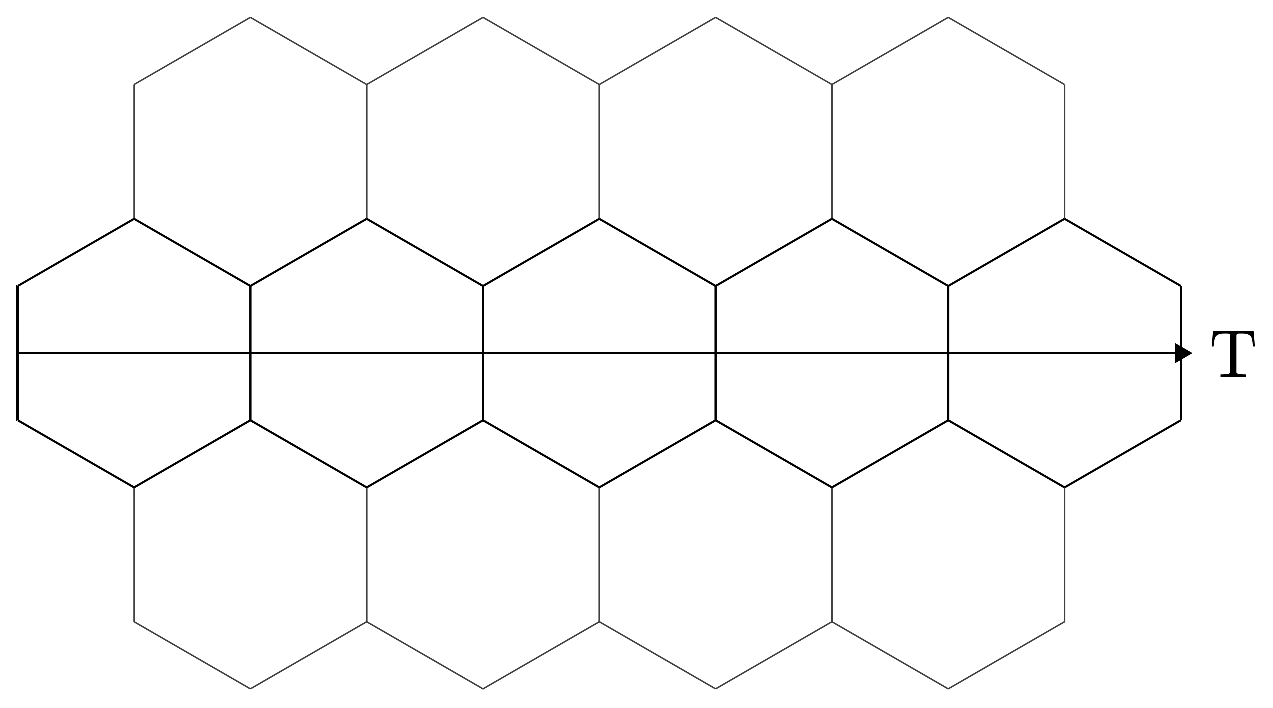
\includegraphics[scale=.25]{./old_fig/Chirality_Armchair.eps}
			\caption{\label{subfig:Armchair}}
		\end{subfigure}%
		~
		\begin{subfigure}[t]{.5\textwidth}
			\centering
			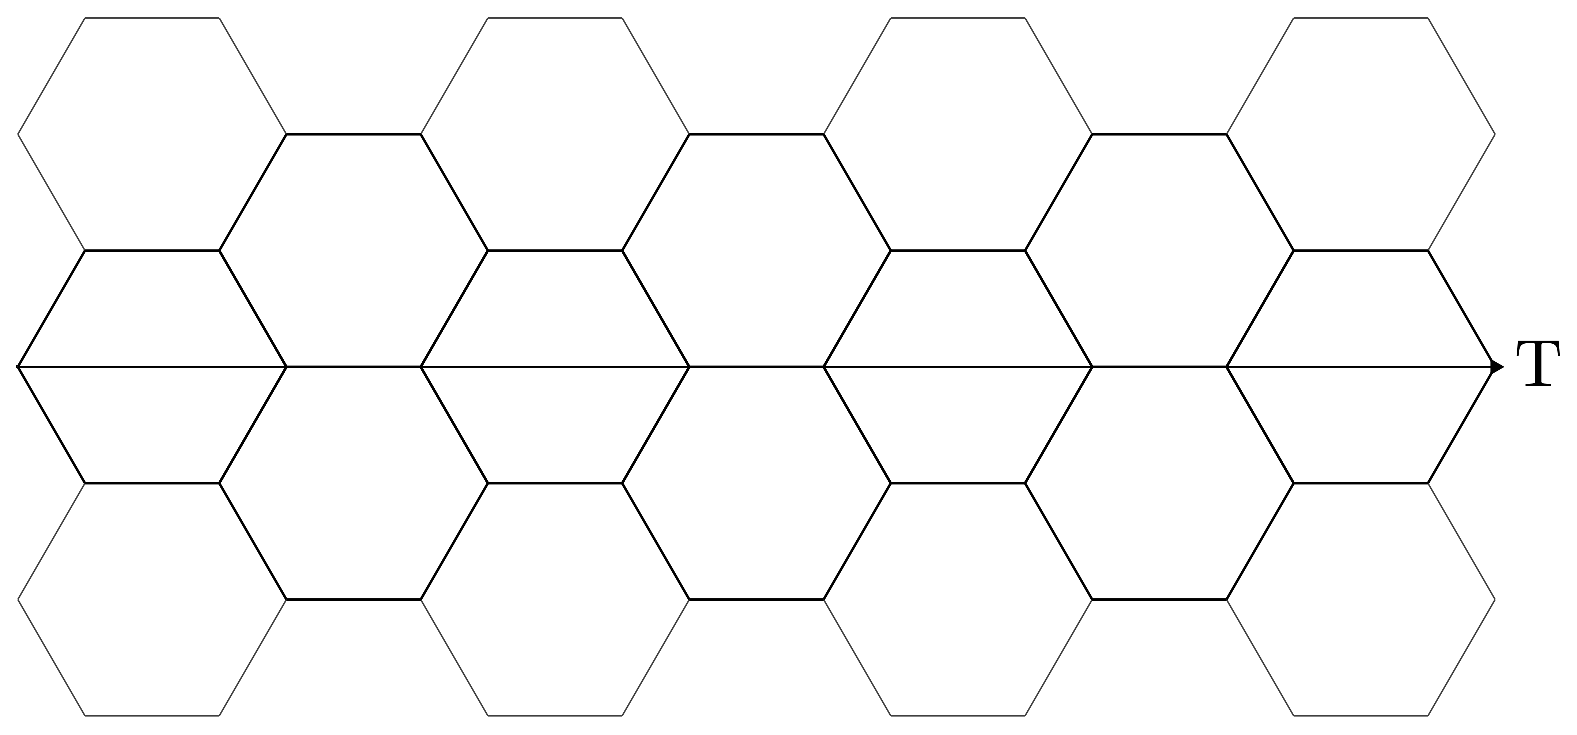
\includegraphics[scale=.25]{./old_fig/Chirality_Zigzag.eps}
			\caption{\label{subfig:Zigzag}}
		\end{subfigure}		
		\caption{Chirality of a CNT can be depicted by how often a hexagonal pattern repeats along a consistent axis. A CNT is (a) armchair if every hexagon is the same, (b) zigzag if the pattern alternates every two hexagons, and chiral otherwise.\label{fig:Chirality}}	
	\end{figure*}
	
\section{Carbon nanotube homogeneous and composite materials}
	
	The macroscopic properties of a homogeneous CNT material are dependent on several factors: purity, porosity, and alignment being a few. A CNT forest, turf, or array is a structure consisting of several CNTs grown from a substrate. A forest is one form of a homogeneous CNT material in that, ignoring the substrate, only the CNTs are present without added polymer or epoxy. One method for producing CNT forests is chemical vapor deposition. CVD has been used in nano-electronic fabrication and is not a new technology. When considered for CNTs it allows for targeted growth on a substrate which is a desirable property for designing and making electronic applications. CVD is thought to have the best potential for commercial success \cite{Nessim2010}. A simplified description of CVD is of a furnace that energizes a gas and substrate (usually with some catalyst) to cause a chemical bonding of gas particles with the substrate. In the case of CNTs the gas consists of hydrocarbons and several different catalysts have been tried and tested. However, the exact mechanism of CNT growth in a CVD process is complicated, between chemical processes depending on the catalyst, ballistics involving the CNT length \cite{Louchev2003}, and temperature of the CVD. The quality of the CNT forest can vary greatly and has been considered more of an art than a science \cite{Nessim2010}.  
	
	Vertically aligned carbon nanotubes (VACNTs) are used in several different application domains. The electrical and thermal conductivity of CNT materials are highly dependent on the alignment bias of the material. Likewise adhesive and optical properties of VACNTs are very dynamic and depend on structure, uniformity, purity and other factors. VACNTs can be used as hydrophobic materials \cite{Lau2003}, dry adhesives \cite{Chen2012}, hologram generators \cite{Montelongo2013}, and nano-workbenches \cite{Gjerde2006}. The adhesive property of VACNTs while simultaneously having low static friction plays a critical role in the hydrophobic, and workbench applications. Xu et al demonstrate a crowding effect of CNT arrays that allows for control of CNT alignment \cite{Xu2012}. The structure of a forest can also be used to spin yarns. A super-aligned array of CNTs can be spun into a yarn of lengths up to centimeters or more \cite{Jiang2002}.
	
	A film of CNTs, with no necessary alignment bias or connection to a substrate, is called buckypaper. Buckypaper is assembled in several ways, including layer-by-layer deposition of functionalized MWCNTs \cite{Lee2008} and ``domino pushing'' of a CNT array. The relative properties of buckypaper is dependent on the assembly method. Wang et al describe the ``domnio pushing'' method as pressing a micropore membrane onto a CNT array. The membrane is pushed by a cylinder with constant pressure from one end to the other of the CNT array causing individual CNTs to collapse in a ``domino'' fashion. The CNTs then stick to the membrane and can be peeled off a silicon substrate and then treated and peeled off the membrane \cite{Wang2008}. A buckypaper assembled with ``domino pushing'' of a highly aligned CNT array will also have an alignment bias, whereas a layer-by-layer deposition will be randomly distributed.

	CNTs are often used as a reinforcing agent in composite materials, for example as dispersed CNTs in an epoxy deposit to improve mechanical strength. A common method of constructing composite materials is through solvents. In a process involving solvents, CNTs are dispersed with a polymer material and then the solvent is carefully evaporated. Uniform dispersion of CNTs is a primary concern for mechanical reinforcement, where ideally the stress applied to a material would be augmented by the strength of the reinforcing tubes \cite{Coleman2006}. There are several composite and reinforcement processes that have been explored which have varying effectiveness to create an improved composite material. Spitalsky et al review several processes and discuss properties of corresponding composites \cite{Spitalsky2010}.

\begin{figure*}[t!]
		\centering
		\begin{subfigure}[t]{.33\textwidth}
			\centering
			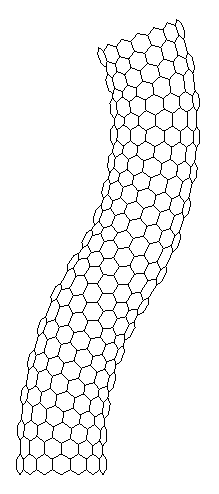
\includegraphics[scale=.25]{./fig/ch1/Nanotube.eps}
			\caption{\label{subfig:Nanotube}}
		\end{subfigure}%
		~
		\begin{subfigure}[t]{.33\textwidth}
			\centering
			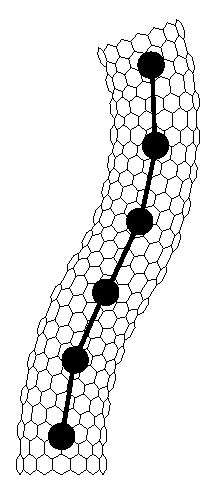
\includegraphics[scale=.25]{./fig/ch1/NanotubeParticle.eps}
			\caption{\label{subfig:NanotubeParticle}}
		\end{subfigure}%
		~		
		\begin{subfigure}[t]{.33\textwidth}
			\centering
			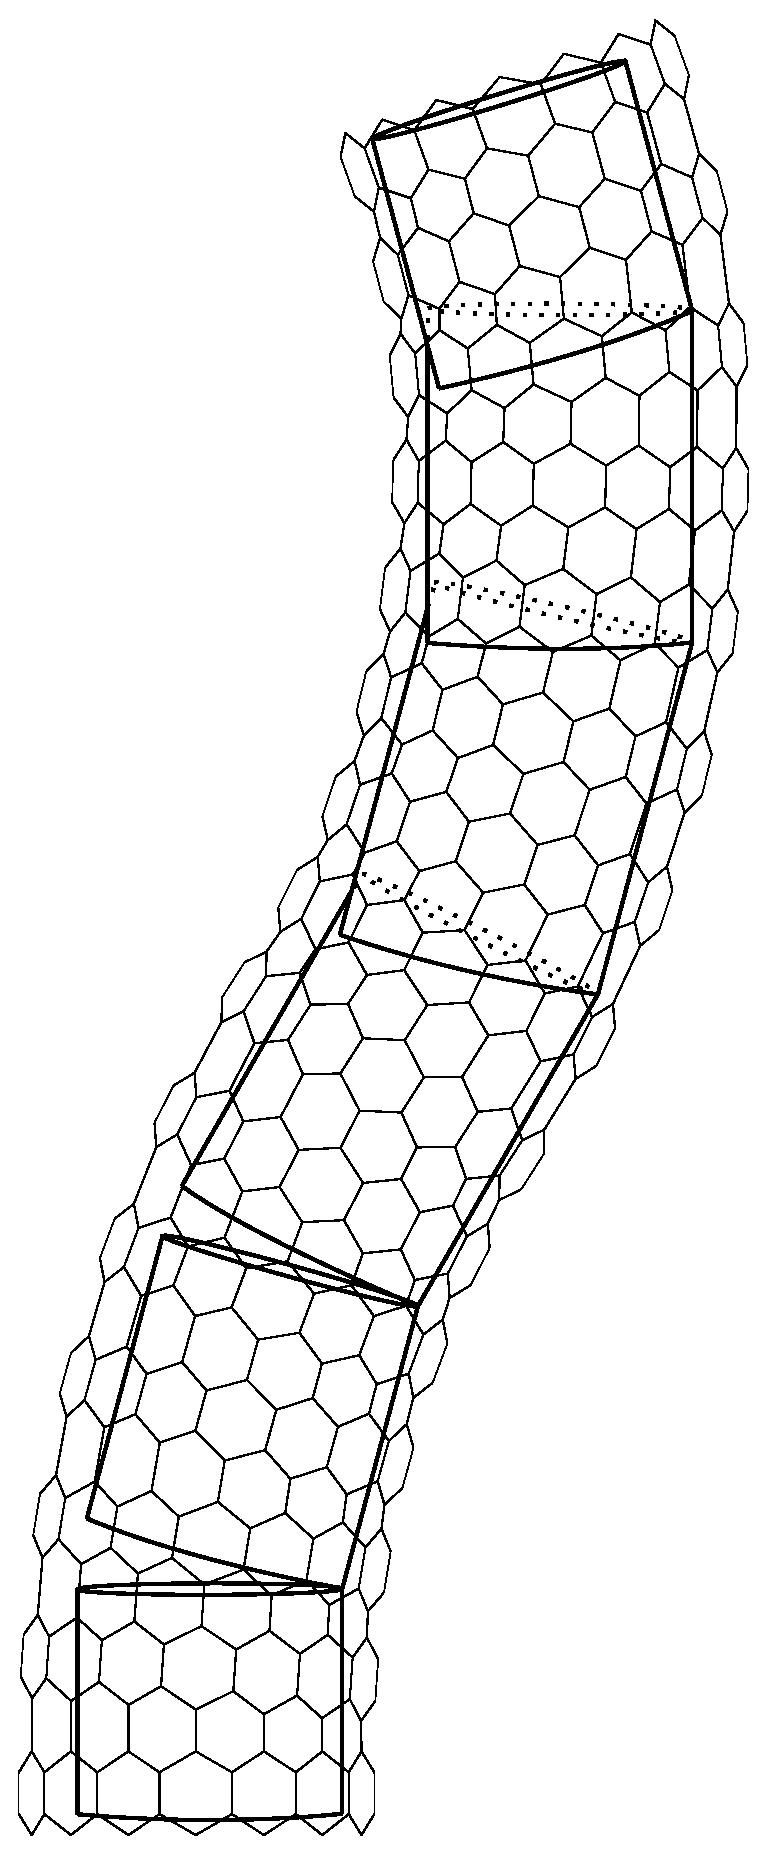
\includegraphics[scale=.25]{./fig/ch1/NanotubeCylinder.eps}
			\caption{\label{subfig:NanotubeCylinder}}
		\end{subfigure}
		\caption{There are several ways to model a CNT with a coarse-grained approach. (a) A CNT under torsional strain can be depicted as (b) a particle bead-spring model of a CNT or (c) a sequence of cylinders model of a CNT. \label{fig:CoarseGrain}}	
	\end{figure*}

\section{Models of buckypaper and fiber materials}

	CNTs in buckypaper can be modelled as individual fibers due to their aspect ratio and flexibility. Indeed, any material consisting of a large volume of CNTs can be thought of as a fiber material. Fiber materials or films are modelled at various length scales. Molecular dynamics takes a small collection of particles and describes their motion with some governing dynamical system for a short period of time. Full atomistic simulations of fiber structures are generally speaking impractical for a large amount of atoms or long time scales. For example, investigation of the heat conductance of a single CNT is a practical consideration for molecular dynamics simulations \cite{Maruyama2003}. In order to investigate longer length and time scales coarse-grained approaches are used. The exact time and length scales that are appropriate for different computational techniques are difficult to quantify. With consistently improving hardware and better algorithms and techniques to handle error propagation the line is steadily shifting. However, qualitatively, molecular dynamics approaches will always be focused on a shorter time scale and smaller systems than coarse-grained approaches which in turn are effective at smaller scales than finite element methods \cite{Muller2002}.
	
	Coarse-grain techniques applied to fiber materials model a collection of atoms as a single particle, encapsulating the motion of an entire fiber as a chain of linked particles, instead of a molecular structure of bonded atoms. The focus of coarse-grained simulations is on the mesoscopic scale, somewhere between 1 nanometer and 1 micrometer.  There are many variations to coarse-grained fibers: the fiber can be thought of as a single rod with an attached particle (or a ``lollipop'') \cite{Buehler2006}, a collection of bead-string links \cite{Li2012} (see Fig.~\ref{subfig:NanotubeParticle}), or a sequence of cylinders \cite{Volkov2008} (see Fig.~\ref{subfig:NanotubeCylinder}). This is a crucial methodology and a cornerstone of this thesis. The ability to garner useful information from a parameterically fitted model that reduces the problems complexity significantly is the ultimate goal. The information loss associated with the coarse-graining can of course not be ignored, but it is not so damaging to make the model useless.
	
	After a model and set of governing equations is developed, the next concern is constructing initial data. When dealing with a fiber material or mesh that consists of hundreds of fibers manual generation of initial data is impractical. Thus appropriate and careful construction of the initial configuration is a primary concern. Preventing fibers from penetrating each other and obtaining a desired volume fraction are two of the issues involved in constructing self-consistent initial data. Dalmas et al modelled fibers as several splines \cite{Dalmas2006}, however there was no inner volume to each fiber due to an effective zero radius of the fibers making it difficult to construct a mesh of a desired volume fraction. Altendorf and Jeulin address this issue with random walks of spheres that can shrink to ``squeeze'' through holes allowing for low porosity \cite{Altendorf2011}. Cranford et al construct an array of fibers independently of the mesh and then sediment each array onto a surface \cite{Cranford2010}.
	
%	The alignment bias of a forest of fibers can be utilized to work with a two dimensional simplification of the array instead of a three dimensional turf. Yang et al apply a load to investigate buckling and adhesion of a forest in two dimensions \cite{Yang2012} and Radhakrishnan et al treat a two dimensional CNT turf as a continuum under nano-indentation \cite{Radhakrishnan2013}.


\section{Models of fiber adhesion}

	%Often there is some potential between atom-like particles in a model of fibril materials. Weak nuclear interactions is a common example, i.e. van der Waals interaction.

	Up until now our focus has been on CNTs, the materials they are associated with, and review of the modelling techniques used to understand them. However, a short-range force at the intermolecular level, van der Waals force, is a critical component of understanding CNTs and how to model them and we have neglected it. Van der Waals force is a combination of several forces, often considered as the sum of intermolecular forces. Weak interactions between molecules can be both repulsive and attractive. Van der Waals interaction has been considered a predominant force in adhesive materials (e.g. dry adhesion of Gecko setae \cite{Autumn2002}), and a van der Waals inspired potential has been used to investigate properties of mesoscopic fibers (e.g. spider silk fibrils \cite{Cranford2013}). The models we consider here are those that consider van der Waals interaction as a critical mechanism for adhesion of a fiber or fiber material. Specifically, the abstracted model we consider thinks of every fiber as interacting via some approximation of van der Waals force.
	
	We can think of our abstraction as a fiber adhesion model. A fiber adhesion model consists of an appropriate model of a fiber material and incorporates adhesion to a given substrate. Although, fiber only adhesion can and has been considered \cite{Li2011}, we will limit ourselves to adhesion involving substrates. Similar to modelling fiber materials without adhesion, molecular dynamics, coarse-grain, and continuum approaches are all relevant. 
	
	Continuum approaches to single fiber models are popular. Fu and Zhang utilized an exact continuum model to investigate peeling of a fiber off a substrate \cite{fu2011}. Majidi introduced a continuum model for fiber adhesion with an upper substrate, in particular focusing on the adhered length of a fiber as a function of the applied normal and shear force \cite{Majidi2009}. Majidi's model was later expanded by He et al to include a coupling effect between shear and normal force \cite{He2012}, and then later to include an axial strain \cite{He2013}. 
	
	To model of several interacting fibers, finite element methods have been used \cite{Radhakrishnan2013}, but the preferred approach seems to be coarse-grained molecular dynamics. Hu et al take a multiscale approach adapting coarse-grained molecular dynamics and finite element method to model an array of fibers between two substrates \cite{Hu2010}. Yang et al investigate a similar problem with only coarse-grained fibers \cite{Yang2012}.
	
	Models of fibers with an adhesive mechanism follow several patterns in the governing energies or forces. Both Hu et al, and Yang et al include at least a bending energy, axial energy, and short-range potential. Hu et al also incorporate a torsional energy, and Yang et al stochastically add springs between neighboring fibers to reinforce the several vertically aligned fibers close to the bottom substrate. If there is an axial energy between particles in a coarse-grained fiber it is usually treated as an extensible spring, however inextensible equivalents also exist. The bending of a fiber is usually determined by the interior angle of contiguous particles along the fiber. Finally, the short-range potential models the van der Waals interaction inter-fiber or between fiber and potentially some other object like a substrate. 

	
\section{Summary}

	We develop a coarse-grain model of a fiber array bounded between a stationary bottom substrate and a free top substrate. The model abstracts any appropriate fiber material, that is such a material that in some physical sense incorporates short-range forces similar to van der Waals force.

\begin{itemize}
	\item {
		In chapter two we introduce the model thoroughly and discuss implementation and simulation concerns,
	}
	\item {
		in chapter three we systematically investigate the effect of loads applied to the top substrate both for compression and detachment of one fiber and then report our findings in a parametric study,
	}
	\item {
		finally in chapter four we report a proof of concept for simulations involving many fibers under the same regime of compression as discussed in chapter three.
	}
\end{itemize}

	With such a simple model we also discover a mode of propagating detachment and note on the inherent level of complexity present in such an abstract and information deprived system.		
		